\section{SCGRA Compilation} \label{sec:scgracompile}
\figref{fig:full-scgra-compilation} depicts the idel SCGRA compilation flow in QuickDough. As shown in the diagram, the compilation esentially is supposed to compile an application compute kernel to an automaticaly customized SCGRA and generate the final bitstream. 

The compilation starts from DFG generation transforming a specified compute kernel probably written in high level language to a DFG. When the DFG is determined, a proper SCGRA configuration is derived through a SCGRA optimizer compromising between the hardware constrain and performance. With both the DFG and SCGRA configuration specified, an operation scheduling algorithm is employed to map the DFG to this SCGRA. Meanwhile, the performance of the DFG running on the SCGRA can be acquired. With these information, it is easy to check whether the design goal is achieved. Usually, it may take multiple iterations to determine an optimized solution. Once the SCGRA configuration is determined, configuration context can also be extracted from the scheduling result. Also we will search the SCGRA library, where there are implementations of various SCGRA configurations. If the implementation of the specified SCGRA conbfiguration is found, then we can integrate the configuration context into the pre-implemented bitstream. If not, corresponding SCGRA HDL model should be generated and implemented before the final bitstream integration. Although it may take a long time to implementat the HDL model, the implementation process will be performed only once as long as the SCGRA configuration is decided.

As mentioned in previous sections, we have not got all the components in \figref{fig:full-scgra-compilation} developed. Currently, we just manually generate the DFG of the compute kernel, and randomly specify two representative SCGRA configuration for all of our benchmark. \figref{fig:base-scgra-compilation} shows the baseline compilation flow, which is the backbone of the ideal compilation flow. Details of the baseline compilation flow is further described in the following sections.

\begin{figure}[H]
\center{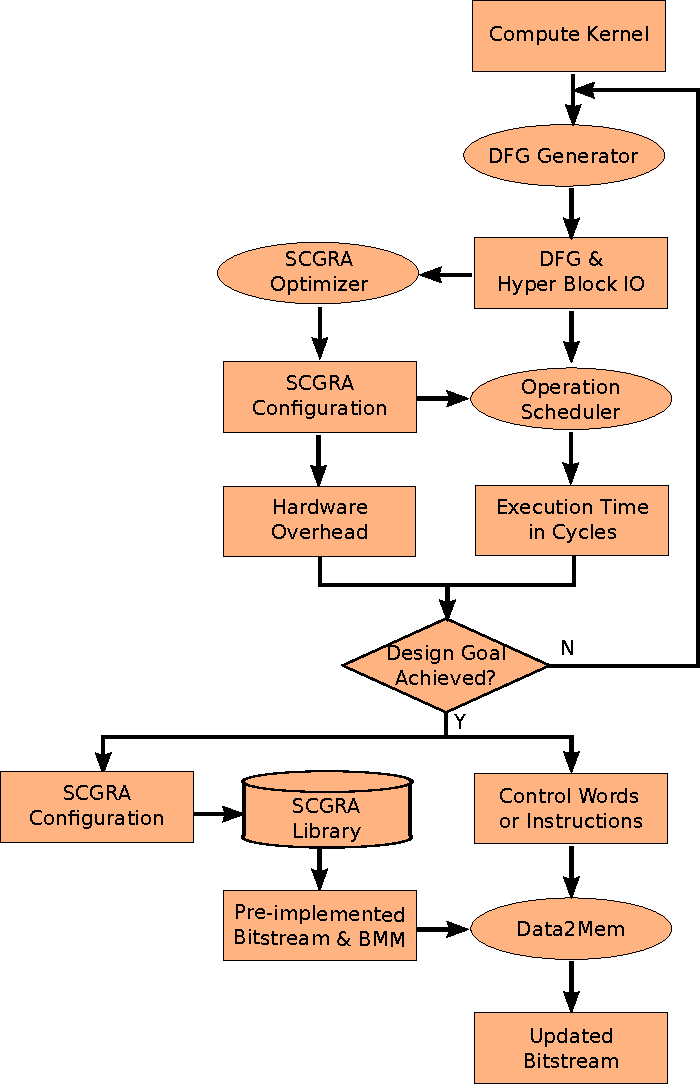
\includegraphics[width=0.7\linewidth]{full-scgra-compile}}
\caption{Ideal SCGRA Compilation Flow}
\label{fig:full-scgra-compilation}
\end{figure}

\begin{figure}[H]
\center{\includegraphics[width=0.5\linewidth]{min-scgra-compile}}
\caption{Baseline SCGRA Compilation Flow}
:\label{fig:base-scgra-compilation}
\end{figure}

\subsection{DFG Generation}
To assist the DFG generation, we developed a group of classes to ease the DFG generation procedurs such as declaring an array of operands and operations, and automatically DFG verification. Eventually, the DFG is represented by three files including operand file, opcode file, and instruction file. The operand file stores details of each operand involved in the DFG such as logical ID of the input/output and data width. The opcode file just defines the meaning of each opcode. The instruction file stores all the operations of the DFG sequentially and each operation is represented as an instruction with destination operand ID, opcode, and source operand ID. Since the accelerator may have data set of multiple SCGRA execution stored in the input/output memory-mapped buffer and data set of differnt SCGRA execution may overlap, we have another io-mapper file to record the IO locations of each SCGRA execution. 
       
\subsection{Operation Scheduling}
In the SCGRA scheduling step, a list scheduling algorithm similar to \cite{colinheart} is adopted to schedule the DFG to the SCGRA infrastructure. It statically schedules the entire DFG on the target SCGRA. Such statically scheduled architecture is crucial in keeping the target SCGRA simple and efficient. To adapt to the proposed SCGRA structure, the scheduling metric is delicately adjusted to compromise the communication cost and load balance. On top of the DFG scheduling, it should also be responsible for generating the addresses for each SCGRA execution using the IO-mapper file. 

\subsection{Bitstream Integration}
The final step of the compilation flow is to incorporate the instruction for each PE obtained from the scheduling stage with the pre-compiled SCGRA bitstream. By design, our SCGRA does not have mechanism to load instruction streams from external memory. Instead, we take advantage of the reconfigurability of SRAM based FPGAs and stored the cycle-by-cycle configuration words using on-chip ROM. The content of these instruction ROMs are embedded in the configuration bitstream. In particular, the organization of the instruction ROM in the place-and-routed SCGRA design is obtained from its XDL file \cite{beckhoff2011xilinx}, which in turn allows us to create the corresponding BMM file. With this BMM file, the encoded instructions collected from the DFG scheduling may then be incorporated into the pre-implemented bitstream using the data2mem tool from Xilinx \cite{data2mem}. While original SCGRA design needs hours to implement, the bitstream updating scheme only costs a few seconds.
